\documentclass[11pt]{article}

\usepackage[margin=1in]{geometry}
\usepackage{amsmath,amssymb,booktabs,graphicx}
\usepackage[hidelinks]{hyperref}

\title{Notes on Reproducing the Single-Bearing EqF Example}
\author{Reproducibility note}
\date{\today}

\begin{document}
\maketitle

\section{Purpose}

This note summarizes a reproduction study of the single-bearing estimation
example from the Equivariant Filter (EqF) paper by van Goor, Hamel, and
Mahony.  The goal is not to dismiss the value of equivariant filtering.
Rather, it is to understand exactly what is being compared, what assumptions
are required for the theory to apply, and what happens when those assumptions
are weakened.

The example is especially useful pedagogically because it is simple enough to
analyze, but subtle enough to expose several common pitfalls in simulation
comparisons.

This is an independent reproduction exercise, not a definitive audit of the
authors' code.  Some discrepancies below may be due to our
implementation choices, unpublished tuning values, or convention differences.
The appropriate conclusion is that the example deserves careful checking and
that the published description is difficult to reproduce exactly.

\section{The Bearing Problem Is Not the Clean IEKF Case}

The strongest invariant-EKF intuition applies when the state itself is a Lie
group and the dynamics are group-affine.  In that setting, an invariant error
can sometimes be mapped through the logarithm to a vector space where the
deterministic error dynamics are exactly linear.

The single-bearing problem is different.  The state is
\[
    \eta \in S^2, \qquad \dot{\eta} = -\Omega^\times \eta,
    \qquad y = c_m \eta .
\]
The sphere is a homogeneous space of \(SO(3)\), but it is not itself a Lie
group.  The action of \(SO(3)\) on \(S^2\) is transitive but not free: many
rotations produce the same bearing.  Thus there is no global bijection
between \(\mathfrak{so}(3)\) and \(S^2\).

The EqF construction still provides a useful equivariant error
\[
    e = \phi(\hat R^{-1},\eta) = \hat R \eta,
\]
and with the paper's normal coordinates the preobserver dynamics are simple.
However, the measurement update remains nonlinear in the chosen error
coordinates.  This is where much of the comparison lives.

\section{Output Linearization: What EqF* Changes}

At the origin, write the normal-coordinate error as
\[
    \epsilon = \begin{bmatrix} a \\ b \end{bmatrix}, \qquad
    \rho = \|\epsilon\|.
\]
The inverse normal chart is
\[
    \eta(\epsilon)
    =
    \begin{bmatrix}
        \cos\rho \\
        -b \frac{\sin\rho}{\rho} \\
        a \frac{\sin\rho}{\rho}
    \end{bmatrix}.
\]
The exact residual is
\[
    r(\epsilon) = \eta(\epsilon) - e_1 .
\]

The standard EqF output matrix gives
\[
    C\epsilon = \begin{bmatrix}0\\-b\\a\end{bmatrix},
    \qquad
    r(\epsilon)-C\epsilon = O(\rho^2).
\]
The EqF* output matrix cancels the second-order term:
\[
    r(\epsilon)-C^*\epsilon = O(\rho^3).
\]
This is a real local advantage.  However, EqF* is also a
measurement-dependent output approximation.  It is not simply the same Kalman
filter applied in better coordinates.  It modifies the output model in a way
that is not applied symmetrically to the EKF baseline in the paper.

This matters.  When comparing filters, readers should ask whether each method
has been given a comparable ``enhancement budget.''  If one method receives a
measurement-dependent correction to its output Jacobian, a fair comparison
should consider analogous corrections for the other methods.

\section{A Sign Inconsistency in the EKF Derivation}

The paper defines the embedded EKF error as
\[
    \tilde\eta := \eta - \hat\eta .
\]
For the norm constraint
\[
    g(\eta)=\|\eta\|^2=1,
\]
the first-order expansion is
\[
    g(\eta)-g(\hat\eta)
    =
    2\hat\eta^\top(\eta-\hat\eta)
    + O(\|\tilde\eta\|^2).
\]
Thus the constraint Jacobian should have the positive sign
\[
    G = 2\hat\eta^\top .
\]
The paper text writes this term with the opposite sign.  The published
Figure~3 EKF heatmap also appears to match the opposite residual sign from the
one stated in the text.  This does not prove that the authors' simulation code
used the wrong sign; it may be only a manuscript or plotting-convention issue.
Nevertheless, it is a concrete inconsistency worth checking in any
reproduction.

Figure~\ref{fig:ekf-sign} compares the two EKF output-linearization sign
conventions.

\begin{figure}[h]
    \centering
    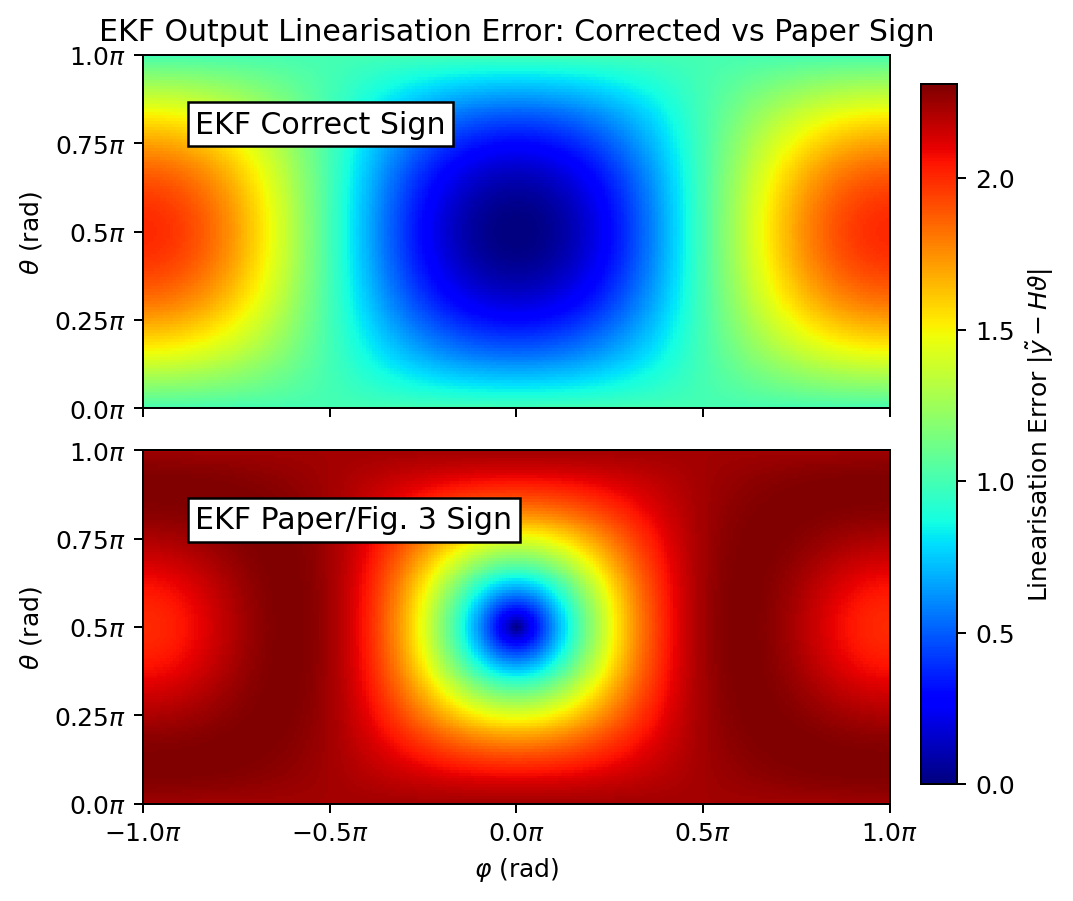
\includegraphics[width=0.72\linewidth]{ekf_linearization_sign_comparison.png}
    \caption{EKF output-linearization error for the mathematically corrected
    sign and the opposite sign convention that appears to match the paper's
    Figure~3.}
    \label{fig:ekf-sign}
\end{figure}

\section{Reproduction Findings}

The paper states the main noise levels and initial distribution, but it does
not publish all numerical tuning values used for the Riccati terms
\(M_\epsilon\), \(N_\epsilon\), or the EKF virtual constraint covariance.
These values matter.  With one reasonable reconstruction of the experiment,
using 500 Monte Carlo trials, the corrected EKF is much closer to EqF* than
the paper's qualitative conclusion suggests.  These numbers should be read as
evidence that the comparison is sensitive to implementation details, not as a
claim that our reconstruction exactly matches the authors' experiment.

\begin{table}[h]
    \centering
    \begin{tabular}{lcc}
        \toprule
        Method & Final median angle error (deg) & Final median Lyapunov value \\
        \midrule
        EqF & 0.2713 & \(9.52\times 10^{-4}\) \\
        EqF* & 0.1956 & \(4.94\times 10^{-4}\) \\
        Adaptive EqF secant, \(k=8\) & 0.1903 & \(4.27\times 10^{-4}\) \\
        Corrected embedded EKF & 0.2081 & \(9.75\times 10^{-4}\) \\
        Adaptive embedded EKF, \(k=8\) & 0.1922 & \(5.90\times 10^{-4}\) \\
        EKF with flipped constraint sign & 0.3582 & \(3.42\) \\
        \bottomrule
    \end{tabular}
    \caption{Representative 500-trial reproduction results.  The adaptive
    methods use the same noise-aware secant blending idea for the EqF and EKF
    output matrices.}
    \label{tab:mc}
\end{table}

Figure~\ref{fig:mc} shows the corresponding Monte Carlo comparison.  The
flipped-sign EKF is included as a diagnostic, not as a recommended algorithm.

\begin{figure}[h]
    \centering
    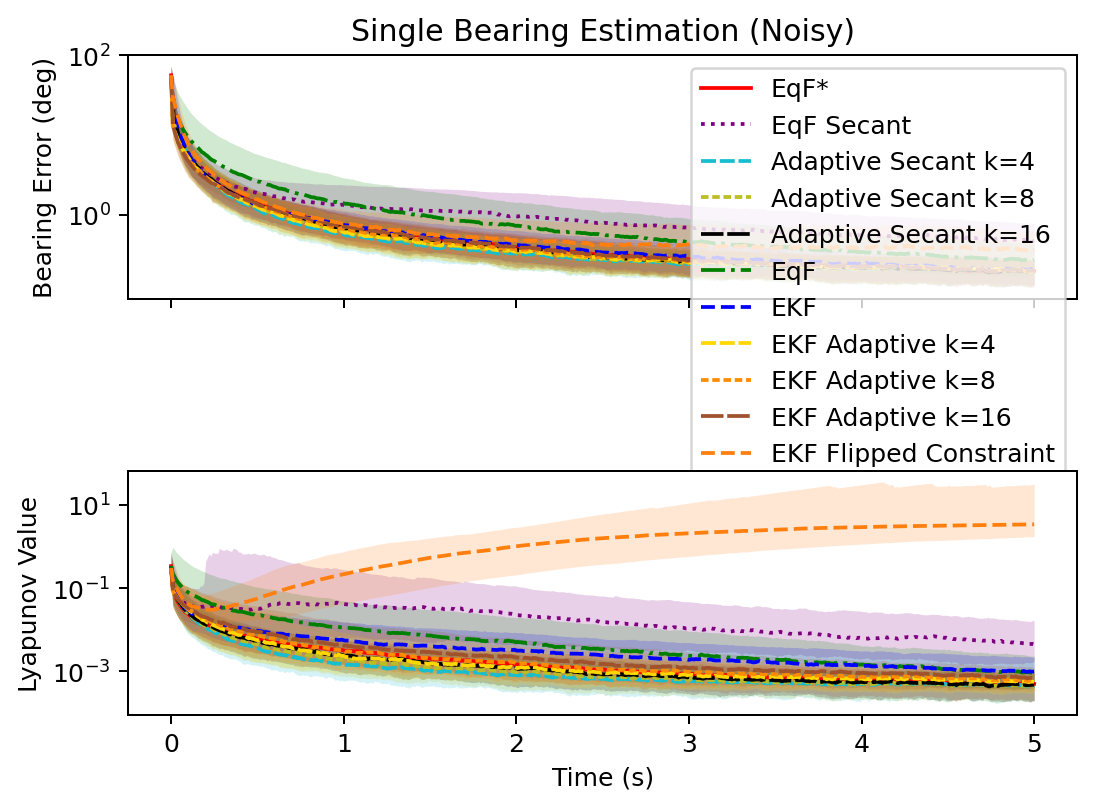
\includegraphics[width=0.82\linewidth]{bearing_monte_carlo_all_comparisons.png}
    \caption{Monte Carlo comparison including EqF, EqF*, corrected EKF,
    flipped-sign EKF, and adaptive output-Jacobian variants.}
    \label{fig:mc}
\end{figure}

\section{What the Adaptive Tests Show}

We tested a measurement-dependent secant matrix \(C_{\mathrm{sec}}\) that fits
the current residual direction.  In the noiseless deterministic approximation,
this can remove residual truncation error along the measured displacement.
But pure secant is rank one and very sensitive to measurement noise near
convergence.

A noise-aware blend
\[
    C_{\mathrm{ad}} =
    (1-\alpha)C + \alpha C_{\mathrm{sec}},
    \qquad
    \alpha =
    \frac{\rho^2}{\rho^2 + k\sigma_y^2},
\]
performed better than pure secant.  This rule gives secant information more
weight when the residual is large relative to measurement noise, and less
weight near convergence.

The important lesson is that this idea is not unique to the EqF.  Applying an
analogous adaptive secant correction to the embedded EKF also improved the
EKF substantially.  Therefore, part of the observed improvement comes from the
output approximation, not only from the equivariant lift.

\section{Conclusions}

\begin{enumerate}
    \item Symmetry and equivariance can produce better error coordinates, but
    the strongest IEKF-style ``exact linear error'' story does not fully apply
    to a homogeneous space such as \(S^2\).

    \item EqF* is a useful output approximation, but it is also an additional
    design choice.  It should not be treated as a purely automatic consequence
    of using a better coordinate system.

    \item The paper appears to contain at least one sign inconsistency in the
    EKF derivation, and the Figure~3 EKF panel appears to use the opposite
    residual sign from the text.  This should be checked against the authors'
    actual simulation code before drawing a stronger conclusion.

    \item Missing simulation settings make exact reproduction difficult.
    In nonlinear filtering, tuning values and discretization choices can
    materially affect the conclusion.

    \item A corrected EKF baseline is much more competitive than the paper's
    qualitative narrative suggests in our reconstruction.  This does not
    invalidate EqF, but it does suggest that the strongest performance claims
    for this particular example should be interpreted with care.

    \item The broader research lesson is constructive: when a method wins, ask
    whether the gain comes from geometry, from an output approximation, from
    tuning, or from an unfair baseline.  Good papers make this separation easy
    to audit.
\end{enumerate}

\end{document}
